\vspace{-2em}
\chapter{Literature Review}
\label{chp:lit-rev}

\section{The rail passenger demand}

The Passenger Demand Forecasting Council - PDFC - is an association of the main stakeholders of the rail industry in Great Britain: train operating companies, Network Rail, Department for Transport, Transport Scotland, the Office of Rail Regulation, Transport for London, the Urban Transport Group, RSSB, HS1, HS2, Rail North, and Welsh Government. The purpose that brings these institutions together is to improve their knowledge about passenger demand \citep{raildeliverygroup}. The motivation is very natural since increasing knowledge about demand allows to create more business opportunities, raise efficiency and profits.

The PDFC's body of knowledge is the Passenger Demand Forecast Handbook - PDFH, which ``summarises over twenty years of research on rail demand forecasting" \citep{raildeliverygroup}. It compiles dozens of studies regarding rail passenger demand and is ``recognised within the industry as the key source of evidence in the area" \citep{raildeliverygroup}.

Therefore, it worths taking a step back to portrait a holistic perspective of the rail demand phenomenon according to the PDFH concepts. The broad elements that affect rail demand, also known as drivers of demand, are presented in Figure \ref{fig:drivers_demand}.

\begin{figure} [H]
\centering
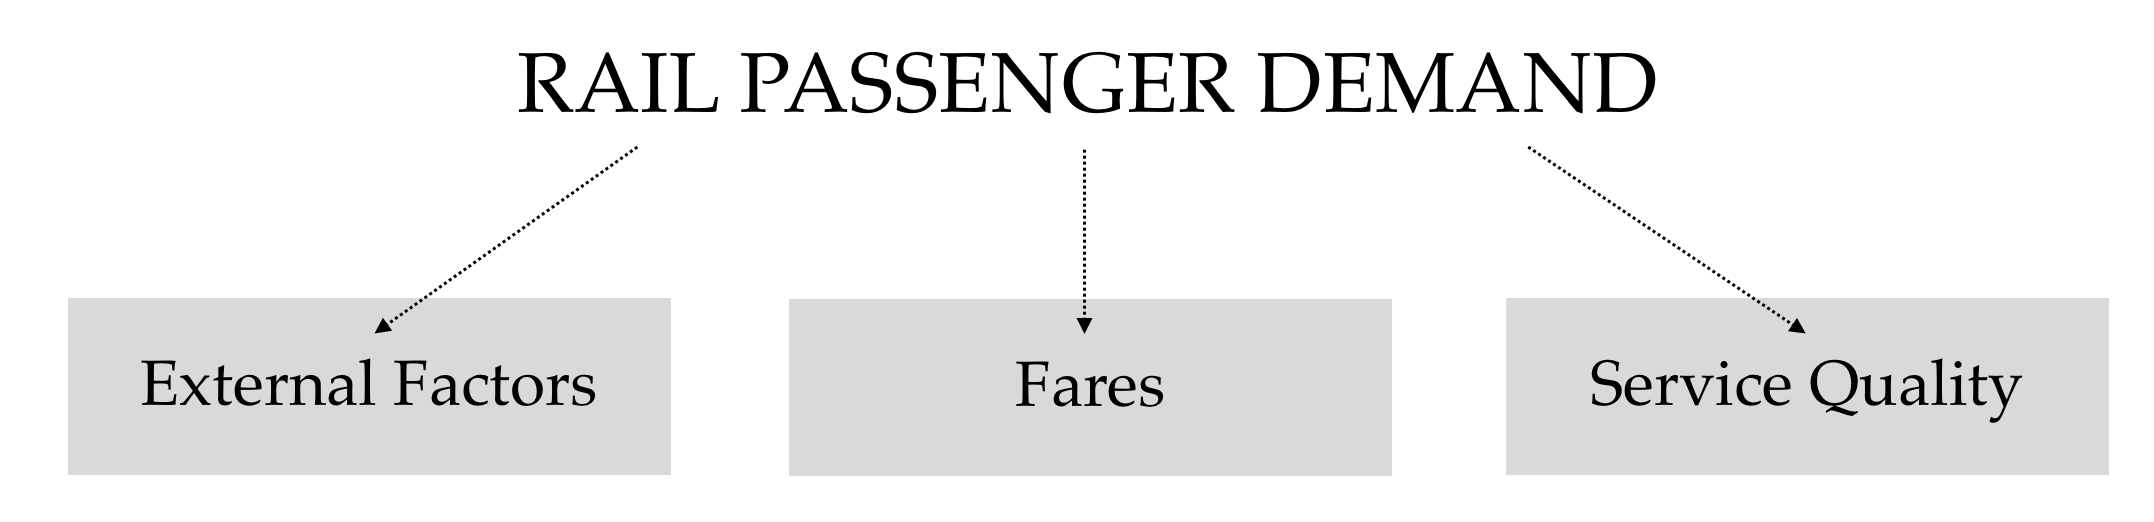
\includegraphics[scale=0.3]{drivers-demand}
\caption{Drivers of rail passenger demand.}
\label{fig:drivers_demand}
\caption*{Source: \cite{pdfh}, Chaper B0, page 1 [adapted]}
\end{figure} 

The first group, as the name says, comprises aspects that are not under control of the train companies. In broad terms, they are related to economic, socio and demographic aspects of the region. Additionally, the availability, quality and cost of competitive modes - car, bus, coaches and air services, are considered.

The second group regards the fares. Despite the evident impact of fares in the demand, the PDFC has been struggling in quantify this impact when it regards how different type of tickets affect their demand, which is the central issue of this work. It will be convenient to extend the discussion about the different types of fares to better interpret the issues around the estimation of the relationship between demand and fares. It will be done in the next section.

% As will be discussed in the sections ahead, several approaches have been tried to quantify these impacts, however, they failed in report coherent and consistent measures. The purpose of this study to apply Bayesian methods to estimate fare elasticity of demand an alternative method to quantify those effects is related to this difficulty

The third group involves the service quality and includes the biggest range of sub elements. The PDFH subsets it as four aspects: 

\begin{enumerate} [label=(\roman*)]
\item Timetable and related features, which covers journey time, frequency and interchange and is usually summarized in the \textit{generalised journey time} measure. 

\item Non-timetable attributes, which in turn comprises overcrowding, rolling stock quality, onboard facilities, station facilities, provision of passenger information, staff and security, cleanliness, advertising and promotion. 

\item Reliability, which covers punctuality and cancellation. 

\item New services and access, which regards the potential demand hold by new services in new or existing routes, new station and also the effects of improving accessibility to stations.
\end{enumerate}

It is noticeable, thus, that the rail passenger demand is considered to be implicated by several factors. For the fare elasticity estimation, however, the demand model is usually simplified to hold fewer elements that are deemed to represent the mass of the covariance of the others drivers of demand. 

Equation \ref{eq:demand_pdfh} presents the short version of demand model.

\begin{equation}
\label{eq:demand_pdfh}
V_{i} = a \; \text{GVA}^g_i \; P^f_i \; \text{GJT}^\gamma_i
\end{equation}
where

$V_i$ is volume of journeys;

$a$ is a constant;

$GVA_i$ is the gross added value;

$P_i$ is the price of the ticket;

$GJT_i$ is the generalised journey time;

$g$ is the GVA elasticity of demand;

$f$ is the price elasticity of demand;

$\gamma$ is the GJT elasticity of demand.
\\[3pt]

This simplification is relevant because for the estimation of individual fare elasticities it is necessary to expand the component price for as many fares as exist, which can make the model inherently complicated. Thus, to keep it simple without losing much information, previous studies have established this simple version \citep{its-systra-report}, which will also be adopted in this study. 

Additionally, as one may notice, the replacement of GDP by GVA is due to the effort to regionalize the income effect across routes \citep{pdfhv5}. Therefore, instead of applying a national GDP, GVA  data is more suitable, since it is available in the NUTS \footnote{Nomenclature of territorial units for statistics.} 3 level.

\section{Rail fares in the UK}

\subsection{Rail fares taxonomy}

\textit{Standard, first class, saver, super saver, single, return, season, peak, off-peak, advance}. Despite one may judge the taxonomy of rail fares to be self-explanatory at a first glance, it can be confusing to structure them into a cohesive system because of the diversity of names and classification used in different types of documents. 

% Appealing to official documents may not help in which regards taxonomy since they usually refer to fares as their terms and conditions, instead of having a classification. This lack of structure is understandable since the regulated fares cover only part of the possible existent fares. Therefore acts, franchising agreements and other official documents do not necessarily mention fares that are defined on a commercial basis; established subject to the strategy of the train operating company.

% It seems, therefore, that the rail taxonomy is a convention usual only to technical reports, even though it is not homogeneous. %For example, Table \ref{tbl:pdfh-fares}, shows the classification adopted in the PDFH. 

% 
\begin{table}[!ht] \centering 
  \caption{Fares Categories in PDFH} 
  \label{tbl:pdfh-fares} 
{\renewcommand\arraystretch{1.25}}
\begin{tabular} {llc}
\toprule
Category         & \multicolumn{2}{p{9cm}}{\raggedright Definition}\\
\hline
First            & \multicolumn{2}{p{9cm}}{\raggedright first class single and return and other first class services.}\\
Standard Open    & \multicolumn{2}{p{9cm}}{\raggedright full fare standard tickets, including standard day, single and return. } \\
Standard Reduced & \multicolumn{2}{p{9cm}}{\raggedright walk-up standard tickets, including saver, super-saver, cheap day return and network away breaks}\\
Standard Apex    & \multicolumn{2}{p{9cm}}{\raggedright includes standard advance purchase tickets. }\\
Seasons          & - \\ 
\bottomrule
\end{tabular}%
\caption*{Source: \cite{pdfh} , Chapter B2, Fares Elasticities, p. 2 [adapted]}
\end{table} 


After gathering different nomenclatures and definitions, they were compiled in Table \ref{tbl:fares-general} as a proposed taxonomy to be adopted in this study to interpret the RUDD's dataset classification. Because season fares will not be part of the scope of this is study they were not considered.


\begin{table}
 \centering 
  \caption{Fares categories and conditions} 
  \label{tbl:fares-general} 
{\renewcommand\arraystretch{1.25}}
\begin{tabular} {ccccccc}
\toprule
Type & \multicolumn{2}{c}{Coverage} & \multicolumn{2}{c}{Conditions}\\ 
\hline
\multirow{2}{*}{\textit{Full}}    & \multicolumn{2}{p{6cm}}{\raggedright \textit{full} or \textit{anytime} or \textit{open}, includes single and return, day single and day return.} & \multicolumn{2}{p{6cm}}{\raggedright Passengers can take any train.}\\
\hline
\multirow{2}{*}{\textit{Reduced}} &  \multicolumn{2}{p{6cm}}{\raggedright \textit{reduced} or \textit{off-peak} or \textit{saver/super saver}, includes single and return, day single and day return for off-peak and supper off-peak.} & \multicolumn{2}{p{6cm}}{\raggedright Passengers can take any off-peak train. Peak time may vary from route to route.}\\
\hline
\multirow{2}{*}{\textit{Advance}} & \multicolumn{2}{p{6cm}}{\raggedright \textit{advance} or \textit{apex}, sold only as single tickets.} & \multicolumn{2}{p{6cm}}{\raggedright Passengers can only take the specific train of the ticket. Must be bought in advance and has limited availability}\\
\bottomrule
\end{tabular}%
\caption*{Source: Own work}
\end{table} 



The three types of fares \textit{Full}, \textit{Reduced} and \textit{Advance} exist in both \textit{First} and \textit{Standard Class}. It will be common to abbreviated these names to their respective initial - $F$, $R$ and $A$, and represent the class as $1$ for \textit{First} and $2$ for \textit{Standard Class}. Thus, concatenating numbers and letters it is possible to make short reference to the fares - $1F$, $1R$, $1A$, $2F$, $2R$, $2A$. An exception for this taxonomy will be the abbreviation $1N$ (\textit{First Class Non-season}) used to refer to the three first class fares together (\textit{Full, Reduced} and \textit{Advance}).

The relevance given to taxonomy is due to the importance of correctly understanding the differences and particularities of tickets to properly interpret the market segmentation and the consumer behaviour. In the same sense, the next section approaches regulatory affairs since they may be useful to contextualise the results.


% the official documents - acts, francising agreements and other regulation documents - do not mention them as structured system of types and classes, but instead they are mentioned as conditions, or characterization, of the service. This may happen due to the fact that the regulated fares covers only part of the possible existent fares. Apart from the regulated fares, the frachisees have the freedom to set other fares in a commercial basis, limited to the conditions of the \textit{Ticketing \& Settlement Agreement} \citep{tsa} - a open boundary to the fare universe. 

% Notwithstanding the possibility of creation of new fares by the franchisees, one can consider the existence of a pattern in their general characteristics since there might be a common need of services with disregard to the franchise. For example, for whichever route that have potential for business clients, the franchise may have interest to have a first class fare. 

% In technical reports is possible to notice classifications which, despite not always structured, bring the ideia of standardization of terms and conditions of fares - \textit{standard, first class, saver, super saver, single, return, season, peak, off-peak} and \textit{advance}.
% % check whether the fares, when created, already receive those kind of names.

% For study purpose, however, the classification from the technical reports may be to wide and some clustering are necessary to allow more simple classification structure. For instance, the reccomendations of fares in the PDFH are based in a segmentation of tickets in five main categories, as shown in Table \ref{tbl:pdfh-fares}.


% By the end of this section, it will be presented an effort to match some names and characteristics of technical reports with te clustered structured of the PDFH. The latter one will be adopted in this study given the available classification of data and also for continuity purpose. 

% Before it however, the next subsection clarifies more aspects of rail fares.

\subsection{Regulated and non-regulated fares}

The rail fares in the Great Britain can be regulated, in which case they are set by the franchising authority, or unregulated, in which case they are set by the train operating companies on a commercial basis \citep{fares-ticketing}. 

According to the last review, run by the Strategic Rail Authority in 2003, there are two groups of regulated fares: the \textit{protected fares} and the \textit{commuter fares} \citep{fares-ticketing}. The regulated fares are set in a price-cap mechanism, where the X may vary according to the objectives of the regulatory policy. Since 2004 it became RPI+1\% \citep{fares-ticketing}.

The \textit{protected fares} seems to serve the broad guidances of regulation policy as they assure reasonable and affordable fares \citep{fares-ticketing}, whilst allows train companies to commercially exploit the route through market segmentation and unregulated fares. According to the taxonomy adopted in the SRA's report \citep{sra-conclusions}, this group of fares comprises:

\begin{itemize}  
\item \textit{Saver returns}, which regards off-peak services, available for most long-distance journeys. In the taxonomy shown on Table \ref{tbl:fares-general} it would be classified as \textit{Reduced}.
\item \textit{Standard returns}, which regards the full-fare and allows the passenger to travel anytime, but only for journeys without the \textit{saver} option. In that taxonomy shown on Table \ref{tbl:fares-general} it would be classified as \textit{Full}.
\item \textit{Weekly season}, others than the ones included in the \textit{commuters fares}. In the taxonomy shown on Table \ref{tbl:fares-general} they would not appear since they regard season fares and others not covered in this study.
\end{itemize}

It is interesting to notice that the regulated fares cover at least one type of ticket that must be available, so a passenger without time restrictions can access the basic service at affordable prices. There is left commercial spots to be price discriminated, targeting users with more strict preferences.

The regulation of \textit{commuter fares} affects mostly season tickets, as well other types as standard single and return within the London Travelcard area or from a pre-defined area of London's suburbs \citep{sra-conclusions}. Because the London area and commuters tickets are out of the scope of this work, they were mentioned just for completeness, but no light will be shed on them.

\section{Fare elasticities of demand}

\subsection{Definition}
The fare elasticities of demand represent the relationship between the demand for a type of fare and the prices of the fares available in the market -  how much the quantity demanded changes when these prices change. It is calculated as the percentage change in quantity demanded by the percentage change in prices, as shown in Equation \ref{eq:elasticity}.

\begin{equation}
\label{eq:elasticity}
\eta = \frac{\% \Delta Q }{\% \Delta P}
\end{equation}
where
% \begin{flalign*}
% \begin{split}
% &\eta \; \text{is the price elasticity of demand} \\
% &Q \; \text{is the quantity demanded} \\
% &P \; \text{is the price}\\
% \end{split}
% \end{flalign*}

$\eta \; \text{is the price elasticity of demand}$

$Q \; \text{is the quantity demanded}$

$P \; \text{is the price}$
\\[3pt]

The fare elasticities of demand may regard the change in the demand of a good $A$ given a change in the price of the good itself, which is called the own-elasticity, shown in Equation \ref{eq:own-elasticity}; or it may regard the change in the demand of a good $A$ given a change in the price of good $B$, which is called cross elasticity, shown in Equation \ref{eq:cross-elasticity}. 

\begin{equation}
\label{eq:own-elasticity}
\eta_{AA} = \frac{\% \Delta Q_A }{\% \Delta P_A}
\end{equation}
where 
% \begin{align*}
% \begin{split}
% &\eta \; \text{is the price elasticity of demand of good $A$ with respect of changes in the price of good $A$} \\
% &Q \; \text{is the quantity demanded of good $A$} \\
% &P \; \text{is the price of good $A$} \\
% \end{split}
% \end{align*}

$\eta$ is the price elasticity of demand of good $A$ with respect to changes in the price of good $A$;

$Q$ is the quantity demanded of good $A$;

$P$ is the price of good $A$.
\\[3pt]


\begin{equation}
\label{eq:cross-elasticity}
\eta_{AB} = \frac{\% \Delta Q_A }{\% \Delta P_B}
\end{equation}
where 
% \begin{align*}
% \begin{split}
% &\eta \; \text{is the price elasticity of demand of good $A$ with respect of changes in the price of good $B$} \\
% &Q \; \text{is the quantity demanded of good $A$} \\
% &P \; \text{is the price of good $B$} \\
% \end{split}
% \end{align*}

$\eta$ is the price elasticity of demand of good $A$ with respect to changes in the price of good $B$;

$Q$ is the quantity demanded of good $A$;

$P$ is the price of good $B$.
\\[3pt]

According to economic theory, the own-elasticity of normal goods, say good A, is expected to be negative indicating that the more the price of good A rises, the lower its demand will be. Conversely, the cross-elasticity of a substitute of a normal good A, say good B, is expected to be positive indicating that the more the price of good B rises, the higher the demand of the good A will be because consumers tend to trade-off to the cheaper good.

The degree of competition between two goods depends upon how close substitutes they are. If two goods are close substitutes, switching from one to another is likely to happen so they become very price sensitive. In other words, if two goods are close substitutes they should have high cross price elasticities.

According to the PDFH, there is a belief that the range of fares covered in this study ($1F$, $1R$, $1A$, $2F$, $2R$ and $2A$) are substitute goods, since they assume that for these fares ``the own elasticity will be negative and the cross elasticities positive" \citep[p.~8, Chapter B2]{pdfh}. 

In fact, they could be regarded as substitutes because ultimately they provide a transport service from one place to another. However, they might differ in the degree of competition, since particularities and specific conditions of each fare are supposed to segregate these markets. 

The extent of this segregation is valuable knowledge. Investigating the fare elasticities of different types of tickets may allow identifying how close these markets really are. 

Additionally, it may reveal different dynamics with regard to the others drivers of demand. For instance, customers of a given type of fare may be more sensitive to service quality than others.

% \begin{align}
% \label{eq:d1f}
% & D_{F} = k{F} \; {P_{F}}^{\eta_{FF}} \; {P_{R}}^{\eta_{FR}} \; {P_{A}}^{\eta_{FA}} \; {P_{f}}^{\eta_{Ff}} \; {P_{r}}^{\eta_{Fr}} \; {P_{a}}^{\eta_{Fa}}\\
% & D_{R} = k{R} \; {P_{F}}^{\eta_{RF}} \; {P_{R}}^{\eta_{RR}} \; {P_{A}}^{\eta_{RA}} \; {P_{f}}^{\eta_{Rf}} \; {P_{r}}^{\eta_{Rr}} \; {P_{a}}^{\eta_{Ra}}\\
% & D_{A} = k{A} \; {P_{F}}^{\eta_{AF}} \; {P_{R}}^{\eta_{AR}} \; {P_{A}}^{\eta_{AA}} \; {P_{f}}^{\eta_{Af}} \; {P_{r}}^{\eta_{Ar}} \; {P_{a}}^{\eta_{Aa}}\\
% & D_{f} = k{f} \; {P_{F}}^{\eta_{fF}} \; {P_{R}}^{\eta_{fR}} \; {P_{A}}^{\eta_{fA}} \; {P_{f}}^{\eta_{ff}} \; {P_{r}}^{\eta_{fr}} \; {P_{a}}^{\eta_{fa}}\\
% & D_{r} = k{r} \; {P_{F}}^{\eta_{rF}} \; {P_{R}}^{\eta_{rR}} \; {P_{A}}^{\eta_{rA}} \; {P_{f}}^{\eta_{rf}} \; {P_{r}}^{\eta_{rr}} \; {P_{a}}^{\eta_{ra}}\\
% \label{eq:d2a}
% & D_{a} = k{a} \; {P_{F}}^{\eta_{aF}} \; {P_{R}}^{\eta_{aR}} \; {P_{A}}^{\eta_{aA}} \; {P_{f}}^{\eta_{af}} \; {P_{r}}^{\eta_{ar}} \; {P_{a}}^{\eta_{aa}}
% \end{align}
% where 
% \begin{align*}
% \begin{split}
% & D_{j} \; \text{are the demand of fare $j$} \\
% & P_{j} \; \text{are the price of fare $j$} \\
% & \eta_{jj} \; \text{are the price elasticity of demand - own and cross, as shown in Equations \ref{eq:own-elasticity} and \ref{eq:cross-elasticity}} \\
% &k_{j} \; \text{are constants.}
% \end{split}
% \end{align*}


\subsection{Difficulties and issues}

As introduced in Chapter \ref{chp:introduction}, estimating fare elasticities is not straightforward.  Indeed, it is being considered the most important area of disagreement on rail demand forecasting" \citep[p.~6]{its-systra-met}. This is so because the traditional estimation of elasticities with the aid of ordinary least squares (OLS) models is hindered by the high correlation of the fares. 

Even though it does not cause bias, the high correlation is a known problem in OLS estimation. When the independent variables are highly correlated it is difficult to isolate individual effects of each variable since most of the variation will be common to both. It leaves the OLS with little information to estimate and because of it, the output might be poor estimates. 

Another way to interpret the high correlation problem regards the fact that when regressors are highly correlated, it is difficult to identify and address the explanatory power among the variables. This fluctuation causes high variances in the estimators causing them not to be precise. It is like their effects in the dependent variable are blurred together and there is low certainty about which one holds which part of it.

In Bayesian inference, however, correlation gains a new perspective. When two predictors are correlated, their coefficients tend to be anti-correlated, which means the bigger one is, the smaller the other will be. In other terms, one can say that ``correlation of predictors causes estimates of their regression coefficients to trade-off" \citep[p.~513]{kruschke2014}. 

That feature can be very useful depending on how the prior distributions are defined in the Bayesian model. When non-informative priors are adopted the blurred effect - the large variance, usual to the OLS  estimation - is reflected in both posterior density of the estimated coefficients. This means that both coefficients will be estimated with a large range of credible values. However, when a strong prior distribution is defined for one coefficient, which means that one is applying a strong belief to constraint its value, it simultaneously constraints the value of the correlated variable, because of their anti-correlation. 

Therefore, when variables are strongly correlated, the constraint applied to one coefficient may ``propagate to the estimates of regression coefficients on other predictors that are correlated with the first" \citep[p.~525]{kruschke2014} and correlation may not be a problem anymore.

There is also the risk of the predictor variables being correlated with omitted variables. In this case, for both methods, it may mislead the interpretation of the coefficients. It worths recovering that an omitted variable, when correlated with a predictor, impacts the predictor estimation to the extent of their correlation \citep{studenmund2011}. Because the remedies to avoid omitted variable bias are related to the theoretical consistency of the model, which was adopted from previous studies, it will not be covered here. 

\subsection{Previous studies}

Several attempts have been tried to solve the issue of estimating fare elasticities applying ticket differentiation. \cite{wardman2003} were the first to estimate consistent own and cross-elasticities, with the correct sign and statistically significant. The successful model applied two theoretical constraints known as ``Slutsky Symmetry" \citep{wardman2003} and ``Dodgson Relationship" \citep{wardman2003}. However, the weakness of this study was the absence of \textit{Advance} ticket, ``although they were very much in their infancy" \citep{its-systra-report}.

A later study of \cite{its-systra-report} have recovered this method to update the evidence and introduce the \textit{Advance} fare in the estimation. However the conclusion was that ``econometric by itself was not able to estimate definitive fare elasticities, but market research would be required in addition" \citep[p.~93]{its-systra-report}.

The mix of revealed preference data with stated preference data turns out to be the more consistent approach. Nevertheless, the authors have concluded that this method has presented a weak performance in some markets segments - especially short distance, which brought vulnerability to it.

As one may notice what all these methods have in common is that they were based on the sampling theory approach. However, ``unrestricted least-squares estimates of own- and cross-price elasticities are often of incorrect sign and unreasonable magnitude" \citep[p.~413]{montgomery1999} and even the usage of contrivances have not achieved satisfactory estimates that can be generalised.  Because of the struggle of the methods attempted so far, it was considered reasonable the exercise to estimate the fare elasticities with the aid of Bayesian regressions.

\section{The bayesian approach}

The Bayesian promise for elasticity estimation is primarily a solution ``to get rid of the wrong signs" \citep[p.~36]{griffiths1988}. The advantage of the Bayesian econometrics is the simple way to incorporate prior information from economic theory \citep{griffiths1988}, which helps to achieve reasonable estimates. 

Beyond that, hierarchical Bayes model has been reported as successful solutions for more complex elasticities estimation \citep{liu2009}. They are useful to problems when it is possible to identify ``meaningful hierarchical structure" \citep[p.~221]{kruschke2014}, in which the parameters can be estimated with the aid of layers of information funnelling from general to specific. For instance, \cite{montgomery1999} have estimated price elasticities of multiple brands and stores with the aid hierarchical model. In this work, the authors are aware of the problem of customizing elasticities estimation from a national level to a regional market, or even store to store, which is the description itself of the hierarchical nature of the problem. The results were reported by the authors as ``reasonable cross-price elasticities estimates while retaining much of the interesting and potentially valuable store-to-store variation" \citep[p.~414]{montgomery1999}. 

As seen, the applications of Bayesian econometrics to elasticity estimation are full of potential. However, because this is an introductory work on the subject,  hierarchical models will be out of scope, and the focus will be strict to the simplest application o Bayesian regression. The next section work on basic concepts of it. 

\subsection{Bayes' theorem}

The Bayesian approach is based on updating the credibility of a prior belief in the light of relevant information, which is the data observed. This abstract rationale becomes a statistical tool through the Bayes' theorem, which is presented in Equation \ref{eq:bayes}.

% \begin{equation}
% \label{eq:bayes}
% 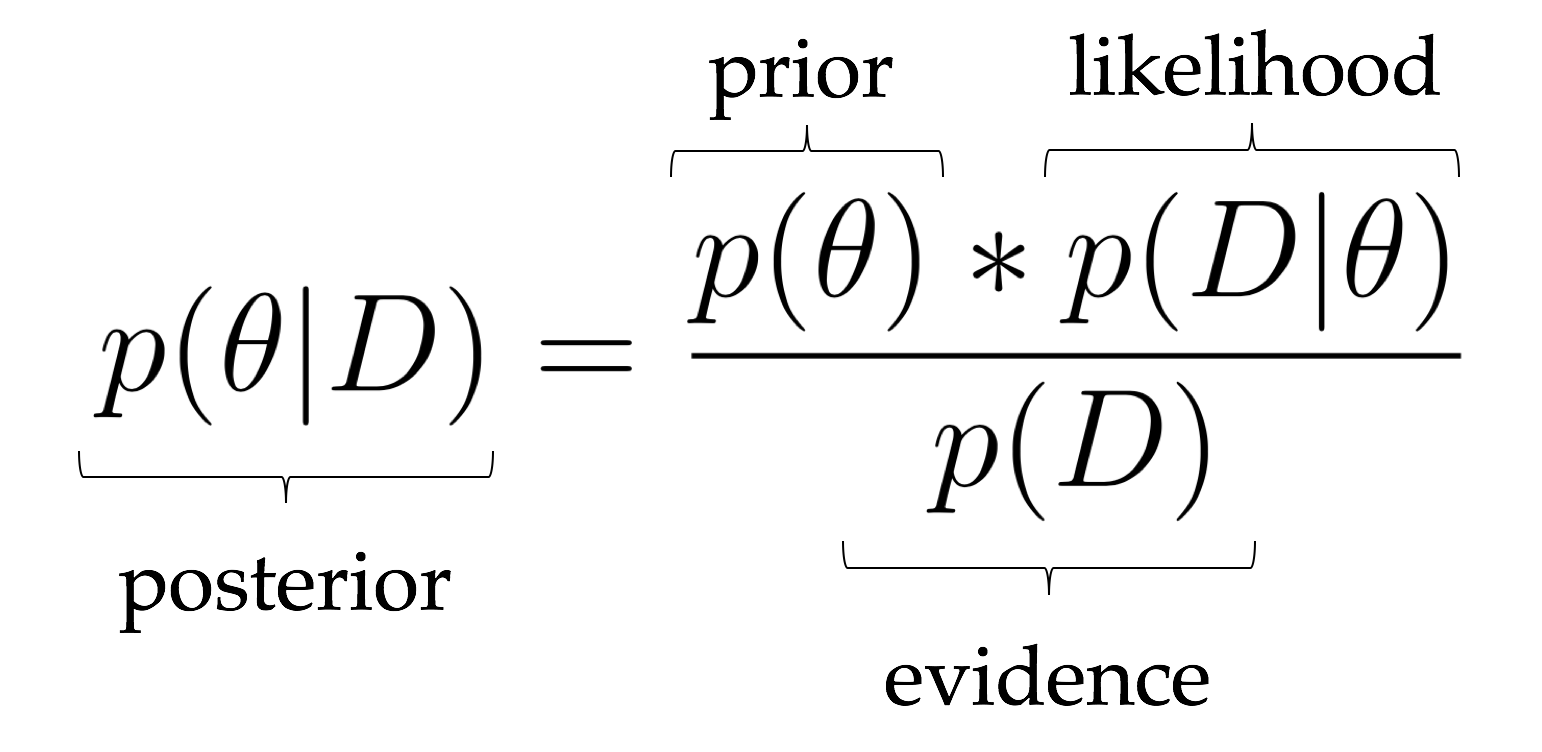
\includegraphics[scale=0.2]{bayes-theorem}
% \end{equation}

\begin{align}
\label{eq:bayes}
  \underbrace{p(\theta \mid D)}_\text{posterior} =  \frac{\overbrace{p(\theta)}^\text{prior} \cdot \overbrace{p(D \mid \theta)}^\text{likelihood}}{\underbrace{p(D)}_\text{evidence}}
\end{align}


where 
\begin{align*}
\begin{split}
&\theta \; \text{is the parameter under study; and} \\
&D \; \text{is tha data observed. It can be thought as a random variable $Y$} \\
& \quad \text{with observations $y_i$}
\end{split}
\end{align*}

The $p(\theta|\text{Data})$ is called the posterior probability density function and represents the updated belief regarding the parameter $\theta$, given an observed data. It is the answer to questions like ``Given the data, what do we know about $\theta$?" \citep{koop2003}.

The $p(\theta)$ is called the prior probability density function. It represents the pre-existent belief regarding $\theta$, unconditional to the observations. The prior belief may be defined due to a theoretical background or to any kind of accumulated knowledge of the subject. 

That is often a critique of the Bayesian approach, being considered a subjective element in the analysis which may pollute the final results. However, a good effect of it is that it demands the researcher to have a prior interpretation of the phenomenon under study and consider reasonable values that it may assume. Indeed, the practice of interpreting a problem before looking at the estimated parameters of a model is highly recommended in the frequentist inference (\cite{gujarati2009}, \cite{kennedy2003}, \cite{studenmund2011}). 

Also, it is important to highlight that the establishment of a prior probability density might not be a mere researcher's opinion. On the contrary, it must be justified to a ``sceptical and scientific audience" \citep{kruschke2012}. Even whether sceptics disagree about the distribution of a prior, there is still the advantage of measure the impact of the disagreement testing the impact of different priors on the final estimate.

The $p(D|\theta)$ represents the likelihood function, which is a function of the parameter $\theta$ for a given data $Y$ assuming that $\theta$ follows a given probability distribution. \cite{gujarati2009} teaches that one may think the likelihood and the probability density function as related functions that are both composed of three parts: i) the parameter under study, $\theta$; the data $Y$, whose observations are $y_i$; and the probability distribution of the parameter under study - how it is expected to behave. It may be useful thinking the function as the analogy of a machine with inputs and outputs. When the input is a possible value of the parameter under study $\theta$, it is the likelihood function, which uses the other two pieces of information to generate the output - the likelihood. Whether the input is the observed data, $y_i$, it is a probability function, which uses the other two pieces of information to generate the output - the (joint) probability of observing $y_i$. 

 % the likelihood ``specifies the probability of values of the predicted variable as a function of the values of the predictor values \citep[p.~421]{kruschke}.

The last element in the Bayes' theorem is the $p(D)$, which represents the observed data. It may be interpreted as the unconditional probability of observing a given $Y$, in the whole universe of possibilities. However, because the interest regards in learning about the parameter under study $\theta$, and $p(D)$ is not related to it, it is usually not considered in the analysis. 

Because of that, it is usually said that the posterior probability density is \textit{proportional} to the prior probability density and the likelihood, as shown in Equation \ref{eq:proportional-bayes} \citep{koop2003}. 

\begin{equation}
\label{eq:proportional-bayes}
p(\theta \vert D) \propto p(\theta) * p(D \vert \theta)
\end{equation}

% An interesting insight about the Bayes's theorem regards the fact that it is based in simple rules of probability. Consider, for instance, two random variables $A$ and $B$, illustrated in Figure \ref{fig:venn-diagram}. 

% \begin{figure}[H]
% \centering
% 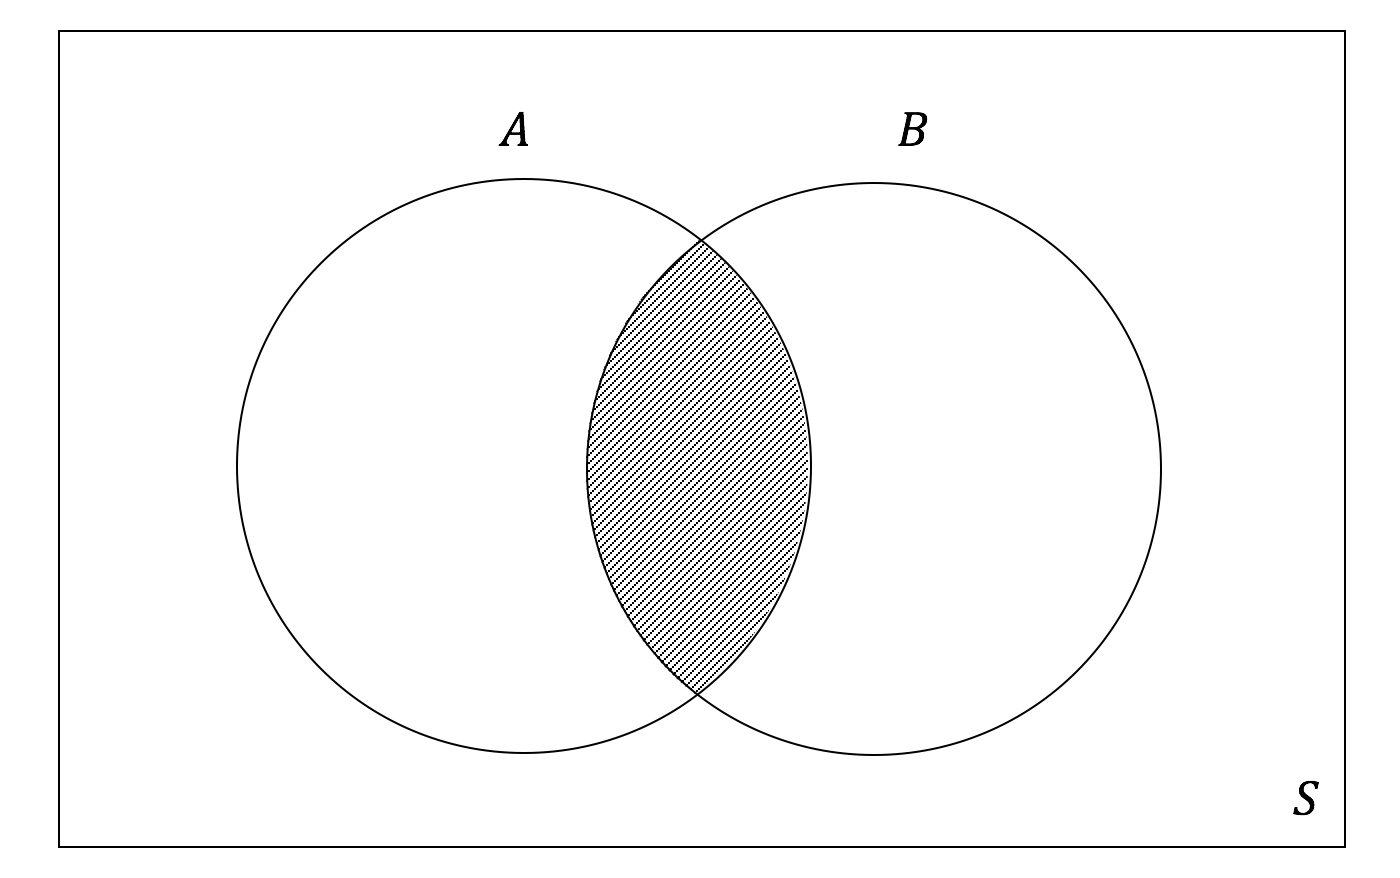
\includegraphics[scale=0.3]{venn-diagram}
% \caption{Venn diagram of sample space $S$ with events $A$ and $B$.}
% \label{fig:venn-diagram}
% \caption*{Source: \cite{montgomery2010} p.24}
% \end{figure} 

% If one is interested in the probability of an event in the shaded area, which means the probability of $A$ and $B$ happening ($ A \cap B$), the rule of the joint probability would state:

% \begin{align}
% \label{eq:joint-prob}
% p(A, B) &= p(B \vert A)*p(B) \quad \text{, or equivalently} \\
% p(A, B) &= p(A \vert B)*p(A)
% \end{align}

% Equaling these two equations, one could achieve a generic format of the Bayes' theorem, as shown in Equation \ref{eq:joint-prob2}, where $A$ would represent $\theta$ and $B$ would represent $D$. 

% \begin{align}
% \label{eq:joint-prob2}
% p(A \vert B) = \frac{p(B \vert A)*p(B)}{p(A)} 
% \end{align}

% At this point, it should be highlighted that the parameter under study in a bayesian inference is random variable. This is the fundamental diference between the bayesian and the frequentist assumptions. Whilst the frequentist approach is chasing the \textit{true} parameter, for instance, the true $\beta$ in a regression, the bayesian assumes that the parameter is a variable itself, and, as such, one should not refer to its \textit{true} value, but to its probability distribution since it can assume a given range of values with different probabilities associated to eachof these values.

\subsection{Running a bayesian regression model}

\textit{Model definition}

Expanding the Bayesian theorem to a practical application in a regression model does not change the Bayes' rationale. However, it may be useful making some explicit considerations since, instead of a unidimensional problem - as presented before, this study will regard a multi dimensional problem because the interest is to estimate several parameters together.

To easily illustrate, consider a regression model with two parameters of interest $\beta_{0}$ and $\beta_{1}$, as given by Equation \ref{eq:regression-model}. 

 \begin{equation}
\label{eq:regression-model}
\hat{y}_{i} = \beta_{0} + \beta_{1}x_{1i}
\end{equation}

Assuming that $\beta_0$ and $\beta_1$ are normally distributed with mean $M_0$ and $M_1$ and standard deviation $S_0$ and $S_1$, respectively, as shown by Figure \ref{fig:prior-likelihood-scheme}, then
\begin{figure}[H]
\centering
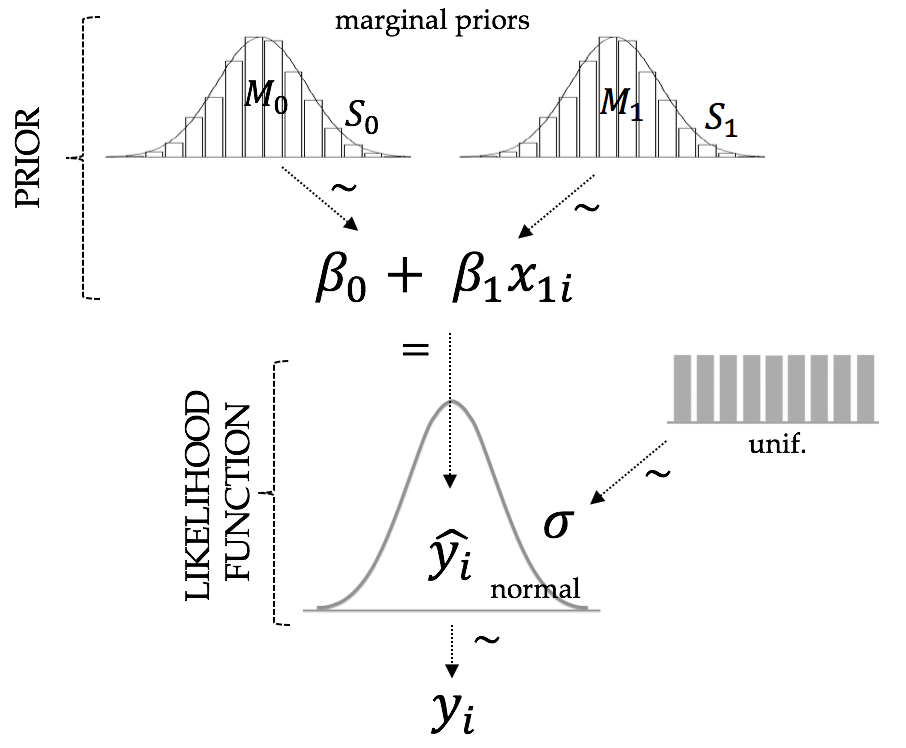
\includegraphics[scale=0.4]{prior-likelihood-scheme}
\caption{Bayesian regression scheme.}
\label{fig:prior-likelihood-scheme}
\caption*{Source: \cite{kruschke2012} p.727 [adapted]}
\end{figure}

\noindent the characterization of the prior probability density would be a three-dimensional space, as shown by Figure \ref{fig:prior-space-prob}. One may notice that the prior is a joint probability of $\beta_0$'s and $\beta_1$'s individual - or marginal - prior probability densities, which integrates to 1.

\begin{figure}[H]
\centering
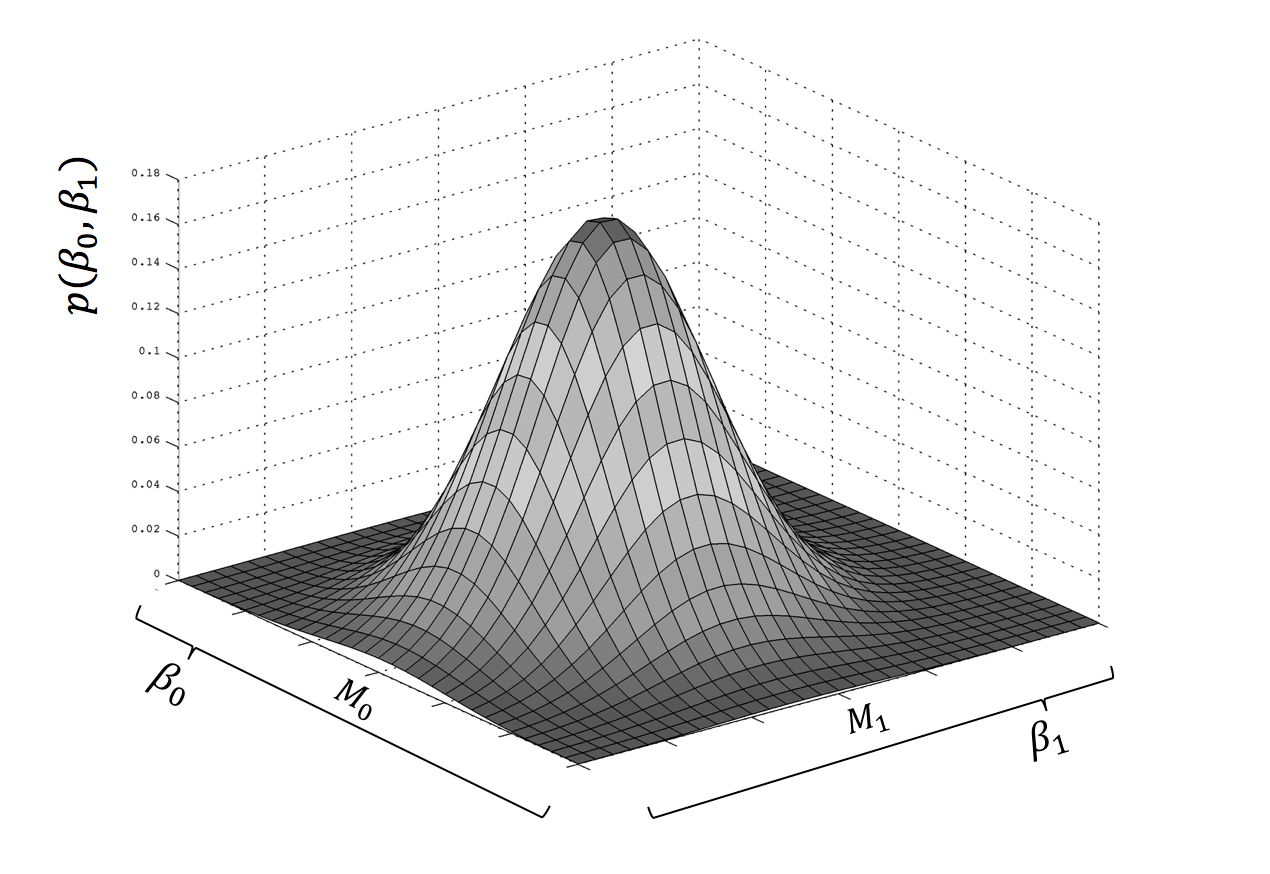
\includegraphics[scale=0.5]{prior-space-prob}
\caption{Prior probability density for parameters $\beta_0$ and $\beta_1$.}
\label{fig:prior-space-prob}
\caption*{Source: Own work}
\end{figure}

The second element to define a Bayesian regression model is the likelihood function, also illustrated in Figure \ref{fig:prior-likelihood-scheme}. In this example, it was assumed that the predicted variable $Y$, which has $y_i$ realizations, is normally distributed with mean $\hat{y}_i$ - which can also be interpreted as $\hat{y}_i = \beta_{0} + \beta_{1}x_{1i}$, and standard deviation $\sigma$. The arrow linking the $\beta$s with the $\hat{y}_i$ shows that there is an equality between it, so $y_i$ is a linear function of the explanatory variables.

A formal way to state this model could be as presented in Equation \ref{eq:model_example}.

\begin{align}
\label{eq:model_example}
\text{y}_i \sim& Normal(\hat{y}_i, \sigma) && \text{[likelihood]} \\
\hat{y}_i =& \beta_{0} + \beta_{1}x_{1i}     && \text{[linear model]}\nonumber\\
\beta_0 \sim& Normal (M_0, S_0) && \text{[prior]}\nonumber\\
\beta_1 \sim& Normal (M_1, S_0) && \text{[prior]}\nonumber\\
\sigma \sim& uniform(a,b) \nonumber          && \text{[prior]}
\end{align}
\\[3pt]

\textit{Estimation of the posterior}

Once defined these elements in the Bayesian regression framework, the result will be a posterior probability density. Analogously to the prior, the posterior will be multidimensional probability space which integrates to 1, similarly to Figure \ref{fig:prior-space-prob} - the exact shape of the posterior will depend on the prior and the likelihood. 

Still analogously to the prior probability density, the posterior is a joint probability space compounded by the marginal posterior distribution of each predictor, in this example $\beta_0$ and $\beta_1$.

The posterior probability density is generated by approximation by collecting from it a large representative sample. This method, called Markov Chain of Monte Carlo - MCMC, is useful when the analytical solution is not possible given the complexity of the posterior distribution \citep{kruschke2014}. ``It is the MCMC algorithms and software, along with faster computer hardware, that allows Bayesian data analysis for realistic applications that would have been effectively impossible 30 years ago"\citep[p.~144]{kruschke2014}.

The core idea of an MCMC lies in the generation of a sequence of samples in the probability space through a random walk process - it may vary among software and algorithms. Each sample is virtually equivalent to a step in the random walk, in which is defined a value for all predictors in the model. For instance, in the example used so far, a step would contain a pair of $\beta_0$ and $\beta_1$ ($\beta_0$, $\beta_1$). 

The random walk is the way the algorithm explores the probability space of possible values. To decide whether or not to accept a step, the algorithm compares the probability of the current step with the probability of the proposed step and applies a decision rule - which may also vary among software and algorithms. These probabilities used in to decide whether or not a proposed step should be accepted are computed from combinations of the prior and the likelihood - recover Equation \ref{eq:proportional-bayes}.

From a given position, the next step is accepted as credible value if the combined probability of the likelihood and the prior is bigger than the current step. If the next step has the lower probability, then a specific decision rule determines whether it is accepted or not. The practical effect is that the MCMC always accepts a step - and keep it as a sample - to explore regions where the probability space has high probability and only accepts part of the steps in regions with lower probability. With long MCMC, there would have been enough steps to provide a good approximation of the posterior probability density. 
